\documentclass[hyperref, a4paper]{article}

\usepackage{geometry}
\usepackage{titling}
\usepackage{titlesec}
% No longer needed, since we will use enumitem package
% \usepackage{paralist}
\usepackage{enumitem}
\usepackage{footnote}
\usepackage{enumerate}
\usepackage{amsmath, amssymb, amsthm}
\usepackage{mathtools}
\usepackage{bbm}
\usepackage{cite}
\usepackage{graphicx}
\usepackage{subfigure}
\usepackage{physics}
\usepackage{tensor}
\usepackage{siunitx}
\usepackage[version=4]{mhchem}
\usepackage{tikz}
\usepackage{xcolor}
\usepackage{listings}
\usepackage{autobreak}
\usepackage[ruled, vlined, linesnumbered]{algorithm2e}
\usepackage{nameref,zref-xr}
\zxrsetup{toltxlabel}
\usepackage[colorlinks,unicode]{hyperref} % , linkcolor=black, anchorcolor=black, citecolor=black, urlcolor=black, filecolor=black
\usepackage[most]{tcolorbox}
\usepackage{prettyref}

% Page style
\geometry{left=3.18cm,right=3.18cm,top=2.54cm,bottom=2.54cm}
\titlespacing{\paragraph}{0pt}{1pt}{10pt}[20pt]
\setlength{\droptitle}{-5em}
%\preauthor{\vspace{-10pt}\begin{center}}
%\postauthor{\par\end{center}}

% More compact lists 
\setlist[itemize]{
    itemindent=17pt, 
    leftmargin=1pt,
    listparindent=\parindent,
    parsep=0pt,
}

% Math operators
\DeclareMathOperator{\timeorder}{\mathcal{T}}
\DeclareMathOperator{\diag}{diag}
\DeclareMathOperator{\legpoly}{P}
\DeclareMathOperator{\primevalue}{P}
\DeclareMathOperator{\sgn}{sgn}
\newcommand*{\ii}{\mathrm{i}}
\newcommand*{\ee}{\mathrm{e}}
\newcommand*{\const}{\mathrm{const}}
\newcommand*{\suchthat}{\quad \text{s.t.} \quad}
\newcommand*{\argmin}{\arg\min}
\newcommand*{\argmax}{\arg\max}
\newcommand*{\normalorder}[1]{: #1 :}
\newcommand*{\pair}[1]{\langle #1 \rangle}
\newcommand*{\fd}[1]{\mathcal{D} #1}
\DeclareMathOperator{\bigO}{\mathcal{O}}

% TikZ setting
\usetikzlibrary{arrows,shapes,positioning}
\usetikzlibrary{arrows.meta}
\usetikzlibrary{decorations.markings}
\tikzstyle arrowstyle=[scale=1]
\tikzstyle directed=[postaction={decorate,decoration={markings,
    mark=at position .5 with {\arrow[arrowstyle]{stealth}}}}]
\tikzstyle ray=[directed, thick]
\tikzstyle dot=[anchor=base,fill,circle,inner sep=1pt]

% Algorithm setting
% Julia-style code
\SetKwIF{If}{ElseIf}{Else}{if}{}{elseif}{else}{end}
\SetKwFor{For}{for}{}{end}
\SetKwFor{While}{while}{}{end}
\SetKwProg{Function}{function}{}{end}
\SetArgSty{textnormal}

\newcommand*{\concept}[1]{{\textbf{#1}}}

% Embedded codes
\lstset{basicstyle=\ttfamily,
  showstringspaces=false,
  commentstyle=\color{gray},
  keywordstyle=\color{blue}
}

% Reference formatting
\newrefformat{fig}{Figure~\ref{#1}}

% Color boxes
\tcbuselibrary{skins, breakable, theorems}
\newtcbtheorem[number within=section]{warning}{Warning}%
  {colback=orange!5,colframe=orange!65,fonttitle=\bfseries, breakable}{warn}
\newtcbtheorem[number within=section]{note}{Note}%
  {colback=green!5,colframe=green!65,fonttitle=\bfseries, breakable}{note}
\newtcbtheorem[number within=section]{info}{Info}%
  {colback=blue!5,colframe=blue!65,fonttitle=\bfseries, breakable}{info}

\newenvironment{shelldisplay}{\begin{lstlisting}}{\end{lstlisting}}

\newcommand{\address}[1]{\href{#1}{\url{#1}}}

\title{Homework 10}
\author{Jiinyuan Wu}

\begin{document}

\maketitle

\paragraph{Problem 1} Kittel Chapter 9 problem 9. Topic: Wannier functions versus atomic orbitals. This problem has you work out some elementary aspects. In general, Wannier functions are highly localized orbitals (exponentially localized), are orthonormal, span the same Hilbert (sub)space as the Bloch states, and the each Wannier function in the "home" unit cell (around origin) translated by a lattice vector is another Wannier function belonging to the unit cell indexed by that lattice vectors (i.e., Wannier functions are translated copies of each other). They are the proper mathematical generalization of atomic orbitals to the crystalline situation.

\paragraph{Solution}  \begin{itemize}
\item[(a)] From 
\begin{equation}
    w\left(\vb*{r}-\vb*{r}_n\right)=N^{-1 / 2} \sum_{\vb*{k}} \exp \left(- \ii \vb*{k} \cdot \vb*{r}_n\right) \psi_{\vb*{k}}(\vb*{r})
\end{equation}
we have 
\[
    \begin{aligned}
        \int \dd[3]{\vb*{r}} w(\vb*{r} - \vb*{r}_n) w^*(\vb*{r} - \vb*{r}_m)
        &= \frac{1}{N} \sum_{\vb*{k}, \vb*{k}'} 
        \ee^{- \ii \vb*{k} \cdot \vb*{r}_n} \ee^{\ii \vb*{k} \cdot \vb*{r}_m}
        \int \dd[3]{\vb*{r}} \psi_{\vb*{k}}(\vb*{r}) \psi_{\vb*{k}'}^*(\vb*{r}) \\
        &= \frac{1}{N} \sum_{\vb*{k}, \vb*{k}'} \delta_{\vb*{k} \vb*{k}'} 
        \ee^{- \ii \vb*{k} \cdot \vb*{r}_n} \ee^{\ii \vb*{k} \cdot \vb*{r}_m} \\
        &= \frac{1}{N} \sum_{\vb*{k}} \ee^{\ii \vb*{k} \cdot (\vb*{r}_m - \vb*{r}_n)} \\
        &= \delta_{mn}.
    \end{aligned}
\]
So when $m \neq n$, we have 
\begin{equation}
    \int \dd[3]{\vb*{r}} w(\vb*{r} - \vb*{r}_n) w^*(\vb*{r} - \vb*{r}_m) = 0.
\end{equation}

\item[(b)] We have 
\[
    \begin{aligned}
        w(x - x_n) &= \frac{1}{\sqrt{N}} \sum_{k} 
        \ee^{- \ii k x_n} \underbrace{\frac{1}{\sqrt{N}} \ee^{\ii k x} u_0(x)}_{\psi_k(x)} \\
        &= \frac{1}{N} u_0(x) \sum_k \ee^{\ii k (x - x_n)} \\
        &= \frac{1}{N} u_0(x) \sum_{i=1}^N \ee^{\ii (x - x_n) \cdot 2\pi i / L} \\
        &= \frac{1}{N} u_0(x) \frac{
            \ee^{\ii (x - x_n) \cdot 2\pi / L} (1 - \ee^{\ii (x - x_n) \cdot 2\pi N / L})
        }{
            1 - \ee^{\ii (x - x_n) \cdot 2\pi / L}
        } \\
        &= \frac{1}{N} u_0(x) \ee^{\ii (x - x_n) \cdot 2\pi / L} 
        \frac{\ee^{\ii (x - x_n) \cdot \pi N / L}}{\ee^{\ii (x - x_n) \cdot \pi / L}}
        \frac{
            \ee^{- \ii (x - x_n) \cdot \pi N / L} - \ee^{\ii (x - x_n) \cdot \pi N / L}
        }{
           \ee^{- \ii (x - x_n) \cdot \pi / L} - \ee^{\ii (x - x_n) \cdot \pi / L}
        } \\
        &= \frac{1}{N} u_0(x) \ee^{\ii (x - x_n) \cdot 2\pi / L} 
        \frac{\ee^{\ii (x - x_n) \cdot \pi N / L}}{\ee^{\ii (x - x_n) \cdot \pi / L}}
        \frac{\sin \pi (x - x_n) N / L}{\sin \pi (x - x_n) / L}.
    \end{aligned}
\]
Note that $L = Na$, and therefore 
\[
    \frac{\sin \pi (x - x_n) N / L}{\sin \pi (x - x_n) / L}
    = \frac{\sin \pi (x - x_n) / a}{\sin \pi (x - x_n) / Na}
    \approx \frac{\sin \pi (x - x_n) / a}{\pi (x - x_n) / Na},
\]
and therefore 
\begin{equation}
    w(x - x_n) = \ee^{\ii \cdot \text{some number}} 
    \cdot u_0(x) \frac{\sin \pi (x - x_n) / a}{\pi (x - x_n) / a},
\end{equation}
and we can just throw away the unitary prefactor and therefore 
\begin{equation}
    w(x - x_n) = u_0(x) \frac{\sin \pi (x - x_n) / a}{\pi (x - x_n) / a}.
\end{equation}

\end{itemize}


\paragraph{Problem 2} Consider a one-dimensional crystal with unit cell of size $a$ with one atom per unit cell. Each atom has one s-orbital (really a Wannier function) centered on each atom. Assume the orbitals are orthonormal.
a) Find the band energy $E(k)$ for a nearest-neighbor tight-binding approximation: the mean energy of the orbital is $A$ and the nearest neighbor tunneling matrix element between orbitals is $-t$ where $t>0$.
b) Find the expressions for the effective mass for electrons and holes at the band extrema.
c) If each atom has one valence electron to donate to the crystal, is the system a metal or insulator? If a metal, what is its $k_F$ ? Answer the same questions if each atom donates two electrons per atom.

\paragraph{Solution} \begin{itemize}
\item[(a)] Following the standard procedure to find the band structure, we have 
\begin{equation}
    \begin{aligned}
        E_{\vb*{k}} &= A + \sum_{\vb*{R}} \ee^{\ii \vb*{k} \cdot \vb*{R}} h(\vb*{R}) \\
        &= A - t \ee^{\ii k a} - t \ee^{- \ii k a} = A - 2 t \cos(ka).
    \end{aligned}
\end{equation}
\item[(b)] The smallest energy is taken when $k = 0$,
and here we have 
\begin{equation}
    \frac{1}{m^*} = \frac{1}{\hbar^2} \pdv[2]{E_k}{k} = 2 t \frac{a^2}{\hbar^2} \cos ka |_{k = 0} = 2 t \frac{a^2}{\hbar^2},
\end{equation}
\begin{equation}
    m^* = \frac{\hbar^2}{2 t a^2}.
\end{equation}
The largest energy is taken when $k = \pm \pi / a$,
and 
\begin{equation}
    \frac{1}{m^*} = \frac{1}{\hbar^2} \pdv[2]{E_k}{k} = 2 t \frac{a^2}{\hbar^2} \cos ka |_{k = \pi / a} = - 2 t \frac{a^2}{\hbar^2},
\end{equation}
\begin{equation}
    m^* = - \frac{\hbar^2}{2 t a^2}.
\end{equation}

\item[(c)] The band can contain $2N$ electrons,
because each $\vb*{k}$ position can host a spin-up electron and a spin-down electron.
So if each atom donates one valence electron,
then the band is half-filled,
so the system is a metal, and
\begin{equation}
    E_\text{F} = A,
\end{equation}
and 
\begin{equation}
    k_{\text{F}} a = \pm \frac{\pi}{2}, \quad k_{\text{F}} = \pm \frac{\pi}{2a}.
\end{equation}
If one atom donates two electrons,
then the band is completely filled and the system is an insulator.

\end{itemize}

\paragraph{Problem 3} Consider an intrinsic semiconductor at finite temperature. The electron and hole mobilities and effective masses are identical in this material. Since electrons move in the conduction band and holes in the valence band (which are different bands), they move independently for this problem.
a) What is the value of the Hall voltage that would be measured in a Hall experiment of a sample of this material?
b) Describe microscopically what the electrons and holes are doing during the Hall effect measurements that then leads to the result of part (a).

\paragraph{Solution} The Hall voltage will be zero, 
because the Hall resistance is zero.
Microscopically, this is because the properties of electrons and holes are exactly the same,
except the former carry negative charge and the latter carry positive charge.
So if a voltage of $U$ is accumulated because of electrons in the conduction band,
then a voltage of $-U$ is also accumulated because of holes in the valence band.
So summing up the contribution of both electrons and holes together,
we find the total voltage is zero.

\paragraph{Problem 4} Calculate the intrinsic conductivity of silicon at room temperature (300 K).  
For concreteness, use the band structure of Si shown in Figure 28.6 of A\&M.  
Take the conduction band effective mass to be 0.19 times the bare electron mass.  
Consider only the heavy hole band with an effective mass of 0.49 times the bare electron mass.  
Use Kittel for any other numerical values that you need.  
To get a sense of whether this is small or large, compare to Cu at room temperature. 

\paragraph{Solution} In intrinsic semiconductors we have
\begin{equation}
    n_i = p_i = 2 \left( \frac{k_{\text{B}} T}{2 \pi \hbar^2} \right)^{3/2} (m_e^* m_h^*)^{3/4} \ee^{- E_g / 2 k_{\text{B}} T}, 
\end{equation}
and 
\begin{equation}
    \sigma = \sigma_e + \sigma_h = e \left( 
        \underbrace{\frac{e \tau_e}{m_e^*}}_{\mu_e} n_i
        + \underbrace{\frac{e \tau_h}{m_h^*}}_{\mu_h} p_i
    \right).
\end{equation}
Here we already know $m_e = 0.19 m_0$, and $m_h = 0.49 m_0$,
and $T = \SI{300}{K}$.
The band structure shown in A\&M tells us $E_g = \SI{1.1}{eV}$.
From Kittel 8.4.1 we know for Si,
the mobility of electrons is \SI{1350}{cm^2/V\cdot s},
while the mobility of holes is \SI{480}{cm^2/V\cdot s},
so the final result is $\sigma = \SI{7.1e-5}{\ohm^{-1} \cdot m^{-1}}$.
On the other hand, the conductivity of Cu is \SI{5.9e7}{\ohm^{-1} \cdot m^{-1}},
so silicon isn't a good conductor compared with copper.

\paragraph{Problem 5} A sample of ultra-pure, intrinsic Ge has been measured to have the following resistance values versus temperature:
\begin{center}
    \begin{tabular}{|l|l|l|l|l|l|l|l|}
        \hline $\mathrm{T}(\mathrm{K})$ & 310 & 321 & 339 & 360 & 383 & 405 & 434 \\
        \hline $\mathrm{R}(\Omega)$ & $13.5$ & $9.1$ & $4.95$ & $2.41$ & $1.22$ & $0.74$ & $0.37$ \\
        \hline
        \end{tabular}
\end{center}
Use this data to determine the energy gap of the material.

\paragraph{Solution} Ignoring the temperature dependence of $\tau$,
we have $\sigma \propto n \propto T^{-3/2} \ee^{- E_\text{g} / 2 k_{\text{B}} T}$,
so 
\begin{equation}
    R = \const \cdot \ee^{E_{\text{g}} / 2 k_{\text{B}} T}.
\end{equation}
By curve fitting (\prettyref{fig:curve-fitting}), we fine 
\[
    \frac{E_{\text{g}}}{2 k_{\text{B}}} = \SI{3254.4}{K},
\]
and 
\begin{equation}
    E_{\text{g}} = \SI{1.08e-19}{J} = \SI{0.56}{eV}.
\end{equation}

\begin{figure}
    \centering
    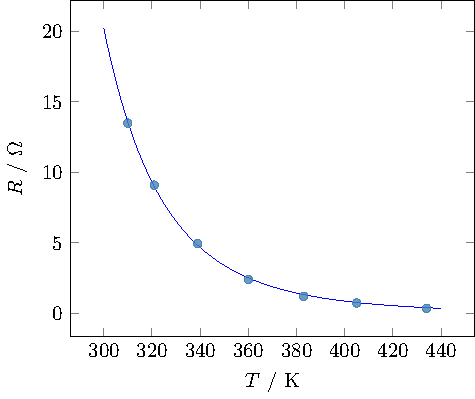
\includegraphics[width=0.4\textwidth]{plots/resistance-fitting-2.pdf}
    \caption{Curve fitting of the relation between $T$ and $R$}
    \label{fig:curve-fitting}
\end{figure}

\end{document}